\documentclass[sigplan,10pt,review]{acmart}\settopmatter{printfolios=true,printccs=false,printacmref=false}
\usepackage[normalem]{ulem} % double underline
\usepackage{fontspec}
\setmonofont{Cabin}
\setmonofont{Comfortaa}
\setmonofont{Latin Modern Mono Light 10 Bold}
% \setmonofont{FreeMono Bold}
\usepackage{listings}
\definecolor{dkblue}{rgb}{0,0.1,0.5} 
\definecolor{lightblue}{rgb}{0,0.5,0.5} 
\definecolor{dkgreen}{rgb}{0,0.4,0} 
\definecolor{dk2green}{rgb}{0.4,0,0} 
\definecolor{dkviolet}{rgb}{0.6,0,0.8}
%\renewcommand*{\ttdefault}{lmss}
\def\lstlanguagefiles{defManSSR.tex,lstlang2.sty}
\lstset{language=SSR, breaklines=false} %flexiblecolumns=false, 
\lstset{moredelim=[is][\uline]{|*}{*|}}
\lstset{moredelim=[is][\uwave]{/+}{+/}}
\lstset{moredelim=[is][\uline]{/*}{*/}}
\lstset{moredelim=[is][\color{dkblue}]{|+}{+|}}

\usepackage[english]{babel}
\usepackage{menukeys}
\newcommand{\derive}[1]{\keys{#1}}

\usepackage{draftwatermark}
%\SetWatermarkText{Draft}

%\usepackage{minted}
%\newminted{coq}{fontsize=\footnotesize,escapeinside=\#\#}
 
%% Conference information
%% Supplied to authors by publisher for camera-ready submission;
%% use defaults for review submission.
\acmConference[PL'18]{ACM SIGPLAN Conference on Programming Languages}{January 14--15, 2019}{Lisbon, Protugal}
\acmYear{2019}
\acmISBN{} % \acmISBN{978-x-xxxx-xxxx-x/YY/MM}
\acmDOI{} % \acmDOI{10.1145/nnnnnnn.nnnnnnn}
\startPage{1}

%% Copyright information
%% Supplied to authors (based on authors' rights management selection;
%% see authors.acm.org) by publisher for camera-ready submission;
%% use 'none' for review submission.
\setcopyright{none}
%\setcopyright{acmcopyright}
%\setcopyright{acmlicensed}
%\setcopyright{rightsretained}
%\copyrightyear{2018}           %% If different from \acmYear

%% Bibliography style
\bibliographystyle{ACM-Reference-Format}


\usepackage{booktabs}
\usepackage{subcaption}

\begin{document}

\title{Deriving proved equality tests in Coq-elpi}
%\titlenote{with title note}
\subtitle{Stronger induction principles for containers in Coq}
%\subtitlenote{with subtitle note}

\author{Enrico Tassi}
\orcid{nnnn-nnnn-nnnn-nnnn}             %% \orcid is optional
\affiliation{
  \institution{Universit\'e c\^ote d'Azur - Inria}
}
\email{Enrico.Tassi@inria.fr}          %% \email is recommended



%% Abstract
%% Note: \begin{abstract}...\end{abstract} environment must come
%% before \maketitle command
\begin{abstract}
We describe a procedure to derive equality tests and their correctness
proofs from inductive type declarations.  Programs and proofs
are derived compositionally, reusing code and proofs derived
previously.  

The key steps are two. First, we
design appropriate induction principles for data types defined
using parametric containers. Second, we
develop a technique to work around the modularity limitations
imposed by the purely syntactic termination check Coq performs
on recursive proofs. 
The unary parametricity translation of inductive data types
turns out to be the key to both steps.

Last but not least, we provide an implementation of the procedure
	for the Coq proof assistant based on the Elpi~\cite{dunchev:hal-01176856} extension language.
\end{abstract}


%% 2012 ACM Computing Classification System (CSS) concepts
%% Generate at 'http://dl.acm.org/ccs/ccs.cfm'.
\begin{CCSXML}
<ccs2012>
<concept>
<concept_id>10011007.10011006.10011008</concept_id>
<concept_desc>Software and its engineering~General programming languages</concept_desc>
<concept_significance>500</concept_significance>
</concept>
<concept>
<concept_id>10003456.10003457.10003521.10003525</concept_id>
<concept_desc>Social and professional topics~History of programming languages</concept_desc>
<concept_significance>300</concept_significance>
</concept>
</ccs2012>
\end{CCSXML}

\ccsdesc[500]{Software and its engineering~General programming languages}
\ccsdesc[300]{Social and professional topics~History of programming languages}
%% End of generated code


%% Keywords
%% comma separated list
\keywords{Coq, Containers, Induction, Equality test, Parametricity
translation}  %% \keywords are mandatory in final camera-ready submission


%% \maketitle
%% Note: \maketitle command must come after title commands, author
%% commands, abstract environment, Computing Classification System
%% environment and commands, and keywords command.
\maketitle

\section{Introduction}

Modern typed programming languages come with the ability of generating
boilerplate code automatically. Typically when a data type is declared
a substantial amount of code is made available to the programmer at
little cost, code such as an equality test, a printing function,
generic visitors etc.  For example the \lstinline+derive+ directive of
Haskell or the
\lstinline+ppx_deriving+ OCaml preprocessor
provide these features for the respective programming language.

The situation is less than ideal in the Coq proof assistant.  It is
capable of synthesizing the recursor of a datatype, that,
following the Curry-Howard isomorphism, implements the induction
principle associated to that datatype. It supports all datatypes,
containers such as lists included, but generates a quite disappointing
principle when a datatype \emph{uses} a container.

For example, let's take the data type rose tree, where \lstinline+U+
stands for a universe (such as \lstinline+Prop+ or \lstinline+Type+):

\begin{minipage}{\textwidth}\begin{lstlisting}
Inductive rtree A : U :=
| Leaf (a : A)
| Node (l : list (rtree A)).
\end{lstlisting}\end{minipage}

\noindent
Its associated induction principle is the following one:

\begin{minipage}{\textwidth}\begin{lstlisting}[numbers=left]
Lemma |+rtree_ind+| : forall A (P : rtree A -> U),
    (forall a : A, P (Leaf A a)) ->
    (forall l : list (rtree A), P (Node A l)) ->
  forall r : rtree A, P r.
\end{lstlisting}\end{minipage}

Remark that the recursive step, line 3, lacks any induction hypotheses
on (the elements of) \lstinline+l+ while one would expect
\lstinline+P+ to hold on each and every subtree. Even a very basic
recursive program such as an equality test cannot be proved correct
using this induction principle.
To be honest, the Coq
user is not even supposed to write equality tests by hand, nor to prove
them correct interactively.  Coq provides two facilities to synthesize
equality tests and their correctness proofs called 
\lstinline+Scheme+ \lstinline+Equality+ and
\lstinline+decide+ \lstinline+equality+. 
The former is fully
automatic but is unfortunately very limited, for example it does not support
containers.  The latter requires human intervention 
and generates a single, very large, term that mixes code and proofs.
% We believe there are deep reasons behind these limitations: in this
% paper we analyse them and propose a solution.

As a consequence, % of the status quo, 
users often need to manually write induction principles,
equality tests and their correctness proofs.
This situation is very unfortunate because the need for the automatic
generation of boilerplate code such as equality tests
is higher than ever in the Coq ecosystem.
All modern formal libraries structure their contents in a
hierarchy of interfaces and some machinery such as type
classes~\cite{Sozeau:2008:FTC:1459784.1459810} or
canonical structures~\cite{10.1007/978-3-642-39634-2_5}
are used to link the abstract library to the
concrete instances the user is working on.
For example the first interface one
is required to implement in order to use the theorems in Mathematical
Components library~\cite{mcb} on a type \lstinline+T+ is the \lstinline+eqType+
one, that requires a correct equality test on \lstinline+T+.

% We see two reasons behind the current state of affairs.
% On one hand the data types one can declare in Coq are very rich,
% making program synthesis hard and proof synthesis even harder.
% On the other hand high level tools
% for meta programming Coq only recently started to appear.
% The derivations described above are coded in OCaml, eg manipulating De
% Bruijn indexes. Experimenting on a derivation is quite expensive.

In this paper we use the framework for meta programming based on
Elpi~\cite{dunchev:hal-01176856,tassi:hal-01637063} developed by the
author and we focus on the derivation of equality tests.
It turns out that generating equality tests is relatively easy,
while their correctness proofs are hard to synthesise, for two reasons. 
The first problem is that 
the standard induction principles generated by Coq, as shown
before, are too weak. In order to strengthen them one needs quite some extra
boilerplate, such as the derivation of the unary parametricity
translation of the data types involved.
The second reason is that termination checking
is purely syntactic in Coq. Rephrased along the Curry-Howard
isomorphism this means that in order to check that the induction
hypothesis is applied to a smaller term, Coq may need to unfold all
theorems involved in the proof. This, in practice, forces all proofs to
be transparent breaking modularity: a statement is no more a contract,
changing its proof script may impact users.

In this paper we describe a derivation procedure for equality tests
and their correctness proofs
where programs and proofs are both
derived compositionally, reusing code and proofs derived previously.
This procedure also confines the termination check issue,
allowing proofs to be mostly opaque.
More precisely the contributions of this paper are the following ones:
\begin{itemize}
\item A technique to confine the termination checking issue out of the
	main proofs. In this paper we apply it to the correctness
	proof of equality
	tests, but the technique is applicable to all proofs 
	that proceed by structural
	induction.

\item A modular and structured process to derive proved equality tests
		and, en passant, stronger
	induction principles for inductive types defined using
	containers.

\item An actual implementation based on the Elpi extension language
	for the Coq proof assistant.
\end{itemize}

\noindent
Straight to the point, by installing the \lstinline+coq-elpi+
package\footnote{See \url{https://github.com/LPCIC/coq-elpi} for the
installation instructions} 
one obtains the following definition, where \lstinline+(reflect P b)+
is a predicate stating the equivalence between a proposition
\lstinline+P+ and a boolean test \lstinline+b+.

\begin{minipage}{\textwidth}\begin{lstlisting}
Definition eq_axiom T f x :=
  forall y, reflect (x = y) (f x y).
\end{lstlisting}\end{minipage}

\noindent
Then by issuing the command \lstinline+Elpi derive rtree+ one gets
the following terms automatically synthesized out of the type
declaration for \lstinline+rtree+:

\begin{minipage}{\textwidth}\begin{lstlisting}
Definition |+rtree_eq+| :
  forall A, (A -> A -> bool) -> rtree A -> rtree A -> bool.

Lemma |+rtree_eq_OK+| : forall A (A_eq : A -> A -> bool),
    (forall a, eq_axiom A A_eq a) ->
  forall t, eq_axiom (rtree A) (rtree_eq A A_eq) t.
\end{lstlisting}\end{minipage}

\noindent
The former is a (transparent) equality test for \lstinline+rtree+.
The latter is a (opaque) proof of correctness for \lstinline+rtree_eq+
under the assumption that the equality test \lstinline+A_eq+ is correct.

The paper introduces the problem in
section~\ref{sec:problem} by describing the shape of an equality test
and of its correctness proof and explaining the modularity problem
that stems for the termination checker of Coq. It then
presents the main idea behind the
modular derivation procedure in section~\ref{sec:idea}.
Section~\ref{sec:elpilang} briefly introduces the Elpi extension language
and section~\ref{sec:code} describes all the bricks composing the
derivation.
% In this paper we systematically omit the
% \lstinline+Definition+ and \lstinline+Lemma+ keywords: terms are given
% a type with \lstinline+:+ and eventually a body with \lstinline+=+.


%%%%%%%%%%%%%%%%%%%%%%%%%%%%%%%%%%%%%%%%%%%%%%%%%%%%%%%%%%%%%%%%%%%%%%%%%%%%%
\section{The problem: equality test proofs meet syntactic termination checking} %%%%%
\label{sec:problem}

Recursors, or induction principles, are not primitive notions in Coq.
The language provides constructors for fix point and pattern matching
that work on any inductive data the user can declare.

For example to test two lists \lstinline+l1+ and \lstinline+l2+ for
equality one first takes in input an equality test \lstinline+A_eq+
for the elements of type \lstinline+A+ and then performs the
recursion:

\begin{minipage}{\textwidth}\begin{lstlisting}[numbers=left]
Definition |+list_eq+| A (A_eq : A -> A -> bool) :=
  fix rec (l1 l2 : list A) {struct l1} : bool :=
    match l1, l2 with
    | nil, nil => true
    | x :: xs, y :: ys => A_eq x y && rec xs ys
    | _, _ => false
    end.
\end{lstlisting}\end{minipage}

\noindent
Coq accepts this definition because
the recursive call is on \lstinline+xs+ that is a syntactically
smaller term, i.e. a subterm, of the input term \lstinline+l1+ (the
argument labelled as decreasing by the \lstinline+{struct l1}+
annotation).

Let's now define the equality test for the \lstinline+rtree+ data type
by reusing the equality test for lists:

\begin{minipage}{\textwidth}\begin{lstlisting}[numbers=left,firstnumber=8]
Definition |+rtree_eq+| B (B_eq : B -> B -> bool) :=
  fix rec (t1 t2 : rtree B) {struct t1} : bool :=
    match t1, t2 with
    | Leaf x, Leaf y => B_eq x y
    | Node l1, Node l2 =>
        list_eq (rtree B) rec l1 l2
    | _, _ => false
    end.
\end{lstlisting}\end{minipage}

\noindent
Note that \lstinline+list_eq+ is called passing as the \lstinline+A_eq+
argument the fixpoint \lstinline+rec+ itself (line 13). In order to
check that the latter definition is sound, Coq looks at the body of
\lstinline+list_eq+ to see weather its parameter \lstinline+A_eq+ is
applied to a term smaller than \lstinline+t1+. Since
\lstinline+l1+ is a subterm of \lstinline+t1+ and since \lstinline+x+
is a subterm of \lstinline+l1+, then the recursive call
\lstinline+(rec x y)+ at line 5 is legit.

This is pretty reasonable for programs. We want both \lstinline+list_eq+
and \lstinline+rtree_eq+ to compute, hence their body matters to us.
The fact that checking the termination of \lstinline+rtree_eq+ requires
inspecting the body of \lstinline+list_eq+ is not very annoying this
time.

On the contrary proof terms are typically hidden to the type checker once
they have been validated, for both performance and modularity reasons.
The desire is to make only the statement of theorems binding, and keep
the freedom to clean, refactor, simplify proofs without breaking
the rest of the formal development. 

For example, lets assume we proved that \lstinline+list_eq+ is
correct.

\begin{minipage}{\textwidth}\begin{lstlisting}[numbers=left]
Lemma |+list_eq_OK+| : forall A (A_eq : A -> A -> bool),
    (forall a, eq_axiom A A_eq a) ->
  forall l, eq_axiom A (list_eq A A_eq) l.
Proof. .. Qed.
\end{lstlisting}\end{minipage}

\noindent
It seems desirable to use this lemma in order to prove the
correctness of \lstinline+rtree_eq+, since it calls
\lstinline+list_eq+.
Unfortunately the following proof is rejected if the body of
\lstinline+list_eq_OK+ is hidden to the type checker:

\begin{minipage}{\textwidth}\begin{lstlisting}[numbers=left,firstnumber=5]
Lemma |+rtree_eq_OK+| B B_eq (HB: forall b, eq_axiom B B_eq b) :
  forall t, eq_axiom (rtree B) (rtree_eq B B_eq) t
:= 
  fix IH (t1 t2 : rtree B) {struct t1} :=
  match t1, t2 with
  | Node l1, Node l2 =>
    .. list_eq_OK (rtree B) (tree_eq B B_eq) IH l1 l2 ..
  | Leaf b1, Leaf b2 => .. HB b1 b2 ..
  | .. => ..
  end.
\end{lstlisting}\end{minipage}

\noindent
We pass \lstinline+IH+, the induction hypothesis, as the
witness that \lstinline+(tree_eq B B_eq)+ is a correct equality test
(the argument at line 11 preceding \lstinline+IH+). 
Without knowing how this argument is used
by \lstinline+list_eq_OK+, Coq rejects the term.

The issue seems unfixable without changing Coq in order to use a more
modular check for termination, for example based on sized
types~\cite{sacchini:pastel-00622429}.
We propose a less ambitious but more practical approach here, that
consists in putting the transparent terms that the termination checker
is going to inspect outside of the main proof bodies so that they can be 
kept opaque.

The intuition is to ``reify'' the property the termination checker wants
to enforce. It can be phrased as ``x is a subterm of t and has the same
type''. More in general we model ``x is a subterm of t with property
P``. Property ``P`` is going to be ``being of the same type`` 
for subterms of ``t`` that are of the same type, while ``P`` 
will be an arbitrary property for terms of an arbitrary type such 
as the elements of a list.

This relation is naturally expressed by the unary parametricity
translation of types~\cite{Wadler:1989:TF:99370.99404}.

%%%%%%%%%%%%%%%%%%%%%%%%%%%%%%%%%%%%%%%%%%%%%%%%%%%%%%%%%%%%%%%%%%%%%%%%%%%%%
\section{The idea: separating terms and types via the unary parametricity translation}
\label{sec:idea}

Given an inductive type \lstinline+T+ we systematically name \lstinline+is_T+
an inductive predicate describing the type of the inhabitants of
\lstinline+T+. This is the one for natural numbers:

\begin{minipage}{\textwidth}\begin{lstlisting}
Inductive is_nat : nat -> U :=
| is_O : is_nat 0
| is_S n (pn : is_nat n) : is_nat (S n).
\end{lstlisting}\end{minipage}

\noindent
The one for a container such as \lstinline+list+ is more interesting:

\begin{minipage}{\textwidth}\begin{lstlisting}
Inductive is_list A (PA : A -> U) : list A -> U :=
| is_nil : is_list A PA nil
| is_cons a (pa : PA a) l (pl : is_list A PA l) :
    is_list A PA (a :: l).
\end{lstlisting}\end{minipage}

\noindent
Remark that all the elements of the list validate \lstinline+PA+.

When a type \lstinline+T+ is defined in terms of another other type
\lstinline+C+, typically a container, the \lstinline+is_C+ predicate
shows up inside \lstinline+is_T+. For example:

\begin{minipage}{\textwidth}\begin{lstlisting}[numbers=left]
Inductive is_rtree A (PA : A -> U) : rtree A -> U :=
| is_Leaf a (pa : PA a) : is_rtree A PA (Leaf A n)
| is_Node l (pl : is_list (rtree A) (is_rtree A PA) l) :
    is_rtree A PA (Node A l).
\end{lstlisting}\end{minipage}

\noindent
Note how line 3 expresses the fact that all elements in the list
\lstinline+l+ validate \lstinline+(is_rtree A PA)+, i.e. they are
rose trees.

Our intuition is that these predicates reify the notion of being
of a certain type, structurally. What we typically write \lstinline+(t : T)+
can now be also phrased as \lstinline+(is_T t)+ as one would do in a
framework other than type theory, such as a mono-sorted logic.

It turns out that the inductive predicate \lstinline+is_T+ corresponds
to the unary parametricity translation of the type \lstinline+T+.
Keller and Lasson in~\cite{keller:hal-00730913} give us an
algorithm to synthesize these predicates automatically.

What we look for now is a way to synthesize
a reasoning principle for a term \lstinline+t+ when 
\lstinline+(is_T t)+ holds.

\subsection{Stronger induction principles for containers} %%%%%%%%%%%%%%%%%%%%%%%%%%%%%

Let's have a look at the standard induction principle of lists.

\begin{minipage}{\textwidth}\begin{lstlisting}
Lemma |+list_ind+| A (P : list A -> U) :
    P nil ->
    (forall a l, P l -> P (a :: l)) ->
  forall l : list A, P l.
\end{lstlisting}\end{minipage}

\noindent
This reasoning principle is purely parametric on \lstinline+A+, no
knowledge on any term of type \lstinline+A+ such as \lstinline+a+ is
ever available.

What we want to obtain is a more powerful principle that lets us choose
some invariant for the subterms of type \lstinline+A+. The one we
synthesise is the following one, where the differences are underlined.

\begin{minipage}{\textwidth}\begin{lstlisting}[numbers=left]
Lemma |+list_induction+| A /*(PA: A -> U)*/ (P: list A -> U):
    P nil ->
    (forall a /*(pa : PA a)*/ l, P l -> P (a :: l)) ->
  forall l, /*is_list A PA l*/ -> P l.
\end{lstlisting}\end{minipage}

\noindent
Note the extra premise \lstinline+(is_list A PA l)+: The
implementation of this induction principle
goes by recursion on the term of this type and finds
as an argument of the \lstinline+is_cons+ constructor
the proof evidence \lstinline+(pa : PA a)+ it feeds to the second premise
(line 3). Intuitively all terms of type \lstinline+(list A)+
validate the property \lstinline+P+, while all terms of type
\lstinline+A+ validate the property \lstinline+PA+.

More in general to each type we attach a property. For parameters we
let the user choose (we take another parameter, \lstinline+PA+ here).
For the type being analysed, \lstinline+list A+ here, we take the
usual induction predicate \lstinline+P+.
For terms of other types we use their unary parametricity translation.

Take for example the induction principle for \lstinline+rtree+.

\begin{minipage}{\textwidth}\begin{lstlisting}[numbers=left]
Lemma |+rtree_induction+| A PA (P : rtree A -> U) :
    (forall a, PA a -> P (Leaf A a)) ->
    (forall l, is_list (rtree A) P l -> P (Node A l)) ->
  forall t, is_rtree A PA t -> P t.
\end{lstlisting}\end{minipage}

\noindent
Line 3 uses \lstinline+is_list+ to attach a property to \lstinline+l+,
and given that \lstinline+l+ has type \lstinline+(list (rtree A))+
the property for the type parameter \lstinline+(rtree A)+ is
exactly \lstinline+P+.
Note that this induction principle gives us access to \lstinline+P+, the
property one is proving, on the subtrees contained in \lstinline+l+.

\subsubsection{Synthesizing stronger induction principles} %%%%%%%%%%%%%%%%%

We postpone a detailed description of the synthesis to
section~\ref{sec:induction}, here we just sketch how to
build the type on the induction principle.

It turns out that the types of the constructors of
\lstinline+is_T+ give us a very good hint on the type
of the induction principle.

The type of the first premise

\begin{minipage}{\textwidth}\begin{lstlisting}
    (forall a, PA a -> P (Leaf A a)) ->
\end{lstlisting}\end{minipage}

\noindent
is exactly the type of the \lstinline+is_Leaf+ constructor

\begin{minipage}{\textwidth}\begin{lstlisting}
| is_Leaf a (pa : PA a) : is_rtree A PA (Leaf A n)
\end{lstlisting}\end{minipage}

\noindent
where \lstinline+(is_rtree A PA)+ is replaced by \lstinline+P+.
The same holds for the other premise: its type can be trivially
obtained from the type of \lstinline+is_Node+.

Our intuition is that the inductive predicate \lstinline+is_T+
provides the same information that typing provides. Induction
principles give \lstinline+P+ on (smaller) terms of the same type,
that would be terms for which \lstinline+is_T+ holds.
Given their inductive nature, \lstinline+is_T+ predicates
are able to propagate the desired property inside parametric
containers.

\subsection{Isolating the syntactic termination check} %%%%%%%%%%%
\label{sec:idea:transparent}

As one expects, it is possible to prove that \lstinline+is_T+
holds for terms of type \lstinline+T+.

\begin{minipage}{\textwidth}\begin{lstlisting}
Definition |+nat_is_nat+| : forall n : nat, is_nat n :=
  fix rec n : is_nat n :=
  match n as i return (is_nat i) with
  | 0 => is_O
  | S p => is_S p (rec p)
  end.
\end{lstlisting}\end{minipage}

\noindent
For containers we can prove this class of theorems
when the property on the
parameter is true on the entire type.

\begin{minipage}{\textwidth}\begin{lstlisting}
Definition |+list_is_list+| : forall A (PA : A -> U),
  (forall a, PA a) -> forall l, is_list A PA l.

Definition |+rtree_is_rtree+| : forall A (PA : A -> U),
  (forall a, PA a) -> forall t, is_rtree A PA t.
\end{lstlisting}\end{minipage}

\noindent
These facts are then to be used in order to satisfy the
premise of our induction principles. 

Going back to our goal, we can build correctness
proofs of equality tests in two steps.
For example, for natural numbers we can generate two
lemmas:

\begin{minipage}{\textwidth}\begin{lstlisting}[numbers=left]
Lemma |+nat_eq_correct+| :
    forall n, is_nat n -> eq_axiom nat nat_eq n :=
  nat_induction (eq_axiom nat nat_eq) PO PS.

Lemma |+nat_eq_OK+| n : eq_axiom nat nat_eq n :=
  nat_eq_correct n (nat_is_nat n).
\end{lstlisting}\end{minipage}

\noindent
where \lstinline+PO+ and \lstinline+PS+ (line 3) stand for
the two proof terms corresponding to the base case and the inductive
step of the proof. We omit them because they play no role in the
current discussion.

For containers we can link the pieces in a similar way.
For example the correctness proof
for the equality test on the \lstinline+(list A)+ data type can be
proved as follows, where again line 7 omits the proof steps for
\lstinline+nil+ and \lstinline+cons+.

\begin{minipage}{\textwidth}\begin{lstlisting}[numbers=left]
Lemma |+list_eq_correct+| A A_eq :
  forall l, is_list A (eq_axiom A  A_eq) l ->
    eq_axiom list A (list_eq A  A_eq)
:=
  list_induction A (eq_axiom A A_eq)
    (eq_axiom (list A) (list_eq A A_eq))
    Pnil Pcons.

Lemma |+list_eq_OK+| A A_eq (HA : forall a, eq_axiom A A_eq a) l :
    eq_axiom (list A) (list_eq A A_eq) l :=
  list_eq_correct l (list_is_list (eq_axiom A A_eq) HA l).
\end{lstlisting}\end{minipage}

\noindent
What is more interesting is to look at the correctness 
proof of the equality test
for \lstinline+rtree+. Note how the induction hypothesis
\lstinline+Pl+
given by \lstinline+rtree_induction+ perfectly fits
the premise of \lstinline+list_eq_correct+.

\begin{minipage}{\textwidth}\begin{lstlisting}[numbers=left]
Lemma |+rtree_eq_correct+| A A_eq :
  forall t, is_tree A (eq_axiom A A_eq) t ->
    eq_axiom (rtree A) (rtree_eq A A_eq)
:=
  rtree_induction A (eq_axiom A A_eq)
    (eq_axiom (rtree A) (rtree_eq Afa))
    PLeaf
    (fun l Pl : is_list (rtree A) 
                  (eq_axiom (rtree A) (rtree_eq A A_eq)) l =>
     .. list_eq_correct (rtree A) (rtree_eq A A_eq) l Pl ..).

Lemma |+rtree_eq_OK+| A A_eq (HA : forall a, eq_axiom A A_eq a) t :
    eq_axiom (rtree A) (rtree_eq A A_eq) t :=
  rtree_eq_correct t (rtree_is_rtree A (eq_axiom A A_eq) HA t).
\end{lstlisting}\end{minipage}

Type checking the terms above does not require any term to be
transparent. Actually they are applicative terms, there is no
apparently recursive function involved.

Still there is no magic, we just swept the problem under the rug.
In order to type check the proof
of \lstinline+rtree_is_rtree+ Coq needs to look at the
proof term of \lstinline+list_is_list+:

\begin{minipage}{\textwidth}\begin{lstlisting}[numbers=left]
Definition |+rtree_is_rtree+| A PA (HPA : forall a, PA a) :=
  fix IH t {struct t} : is_rtree A PA t :=
  match t with
  | Leaf a => is_Leaf A PA a (HPA a)
  | Node l =>
      is_Node A PA l
        (list_is_list (rtree A) (is_rtree A) IH l)
  end.
\end{lstlisting}\end{minipage}

\noindent
As we explained in section~\ref{sec:problem} Coq needs to know the
body of  \lstinline+list_is_list+ in order to agree that the argument
\lstinline+IH+ is only used on subterms of \lstinline+t+.

Even if we can't make the problem disappear (without changing the way Coq
checks termination), we claim we confined the termination checking issue
to the world of reified type information. The transparent proofs of
theorems such as \lstinline+T_is_T+ are separate from the other, more
relevant, proofs that can hence remain opaque as desired.

%%%%%%%%%%%%%%%%%%%%%%%%%%%%%%%%%%%%%%%%%%%%%%%%%%%%%%%%%%%%%%%%%%%%%%%%%%%
\section{Elpi: an extension language for Coq} %%%%%%%%%%%%%%%%%%%%%%%%%%%%%%%%%%%%%%%%%%%%%%%%%%
\label{sec:elpilang}

Elpi~\cite{dunchev:hal-01176856} is a dialect of
$\lambda$Prolog~\cite{miller_nadathur_2012}, an higher order logic
programming language. Elpi can be used as an extension language for
Coq~\cite{tassi:hal-01637063} in order to develop new commands in a programming
language that has native support for bound variables.

Coq terms are represented in $\lambda-$tree syntax
style~\cite{10.1007/3-540-44957-4_16} (sometimes also called
Higher Order Abstract Syntax) reusing the binders of the programming
language to represent the ones of Coq.
For example, the
term \lstinline+(fun x => fact x)+ is represented as
\lstinline+(lam (fun x, app["fact",x]))+. 
We say that \lstinline+app+ and \lstinline+lam+ are object level term
constructors standing for iterated (n-ary) application and unary lambda
abstraction; \lstinline+"fact"+ is a constant and \lstinline+x+ is a
variable bound by \lstinline+fun x,+ that is the binder
of the programming language.  \footnote{In this paper we simplify
a little the embedding and use strings to represent Coq constants.
In reality
global constants are explicit nodes, e.g. \lstinline+nat+,
being an inductive type,
is written \lstinline+(indt "Coq.Init.Datatypes.nat")+,
while \lstinline+fact+, being a constant,
is written \lstinline+(const "Coq.Arith.Factorial.fact")+.}

Programs are
organized in clauses that represent both a data base of known facts
and a set of rules to derive new facts out of known ones.
For example one could use a relation named \lstinline+eq-db+
to link a type to its equality test.

\begin{minipage}{\textwidth}\begin{lstlisting}
eq-db "nat" "nat_eq".
eq-db (app["list", B]) (app["list_eq", B, B_eq]) :-
  eq-db B B_eq.
\end{lstlisting}\end{minipage}

The first clause is a fact stating that
\lstinline+nat_eq+ is the equality test for type
\lstinline+nat+.
The second clause is an inference one and reads: the equality test
for \lstinline+(list B)+ is \lstinline+(list_eq B B_eq)+ \emph{if}
\lstinline+B_eq+ is the equality test for \lstinline+B+.

The \lstinline+eq-db+ data base can be queried for
an equality test for, say, \lstinline+(list nat)+ as follows:

\begin{minipage}{\textwidth}\begin{lstlisting}
eq-db (app["list", "nat"]) F.
\end{lstlisting}\end{minipage}

\noindent
where \lstinline+F+ is a variable to be filled in.
By chaining the two clauses Elpi answers:

\begin{minipage}{\textwidth}\begin{lstlisting}
F = app["list_eq", "nat", "nat_eq"]
\end{lstlisting}\end{minipage}

\noindent
that read back in the Coq syntax is
\lstinline+(list_eq nat nat_eq)+, the desired
equality test.

It is worth recalling out that in $\lambda$Prolog the set of clauses
is dynamic: a program is allowed to add clauses inside
a specific scope (typically the one of a binder) and the runtime
collects them when the scope ends. As we will see, this feature
is useful when a derivation takes place under an hypothetical
context, e.g. when one assumes a parameter \lstinline+A+ and
an equality test \lstinline+A_eq+.
No other feature of the Elpi language is relevant to this paper.

Finally, the integration of Elpi in Coq exposes to the extension
language primitives to access the logical environment, e.g.
to read an inductive data type declaration; to declare a
new inductive type; to define a new constant; etc\ldots

%%%%%%%%%%%%%%%%%%%%%%%%%%%%%%%%%%%%%%%%%%%%%%%%%%%%%%%%%%%%%%%%%%%%%%%%%
\section{Anatomy of the derivation} %%%%%%%%%%%%%%%%%%%%%%%%%%%%%%%%%%%%%%%%%%%%%%%%%%%%%%%%
\label{sec:code}

The structure of the derivation is depicted in the following diagram.
Each box represents a component deriving a complete term.
An arrow from component A to component B tells that the terms
generated by B are used by the terms generated by A. The interfaces
between these components are indeed types: one can replace the work
done by each component with a few hand written terms, if necessary.

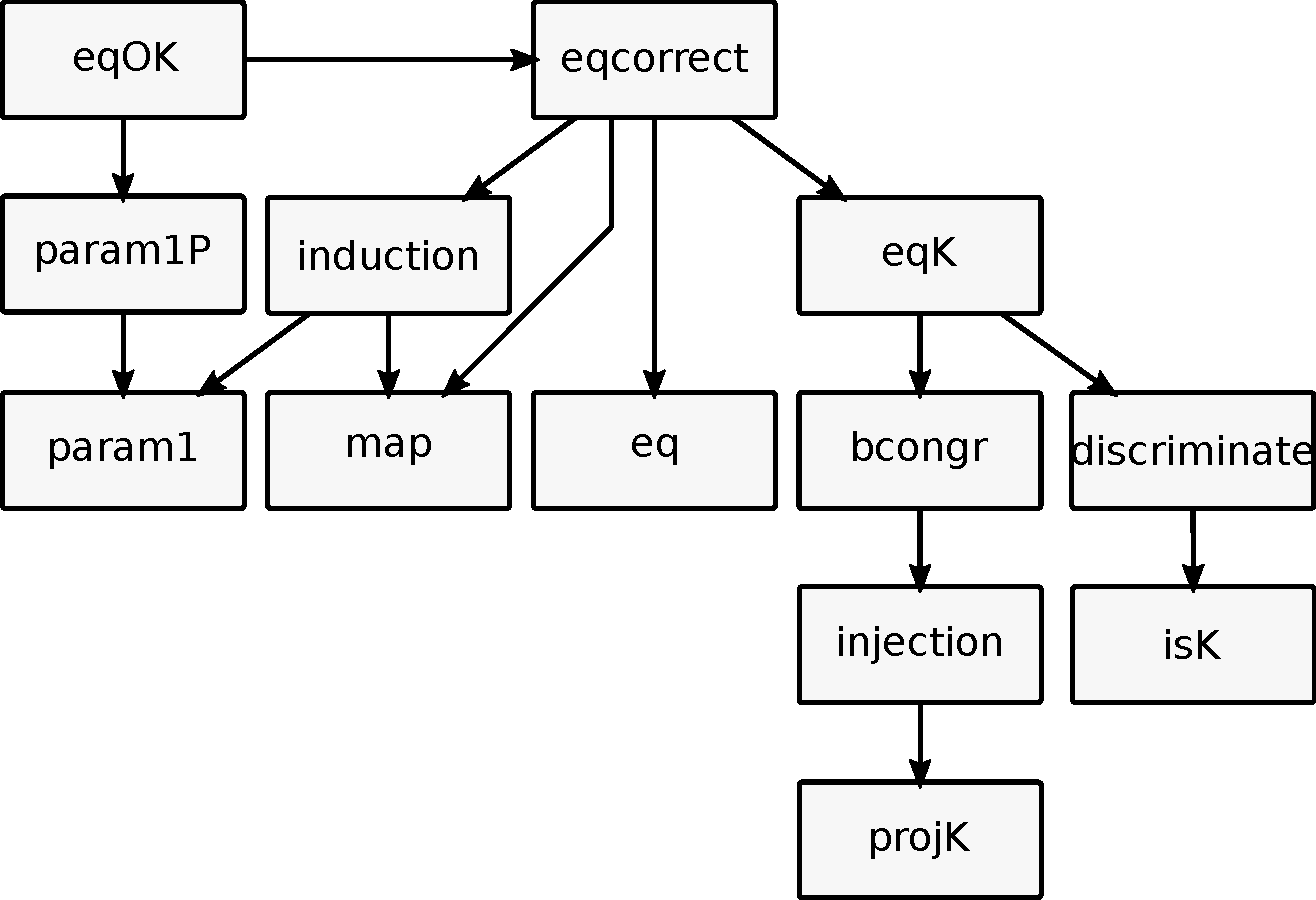
\includegraphics[width=0.45\textwidth]{derive.pdf}

The \derive{eq} component is in charge of synthesizing the program
performing the equality test.
% Recursion is performed on the first
% term; then the two terms are inspected via pattern matching. If the
% constructors are different the output is false, otherwise the
% results of the recursive calls on the subterms are composed using
% boolean conjunction.

The correctness proof generated by \derive{eqcorrect} goes by induction on
the first term of the two being compared and then goes on
in a different branch for each constructor K. 
The property being proved by induction is expressed
using \lstinline+eq_axiom+ that, as we will detail in
section~\ref{sec:reflect} is equivalent to a double implication.
The \derive{bcongr} component proves that the property is preserved
by equal contexts, that is when the two terms are built using the
same constructor. When they are not the program must return false
and the equality be false as well: this is shown by \derive{eqK},
that performs the case split on the second term. The no confusion
property of constructor is key to this contextual reasoning.
\derive{projK} and \derive{isK} generate utility functions that
are then used by \derive{injection} and \derive{discriminate} to
prove that constructors are injective and different.
As we sketched in the previous sections the unary parametricity
translation plays a key role in expressing the induction
principle. The inductive predicate \lstinline+is_T+ for an inductive
type \lstinline+T+ is generated by \derive{param1} while
\derive{param1P} shows that terms of type \lstinline+T+ validate
\lstinline+is_T+. \derive{map} shows that \lstinline+is_T+ is a
functor when \lstinline+T+ has parameters. This property is both
used to synthesize induction principles and also to combine the
pieces together in the correctness proof.
The \derive{eqOK} component hides the \lstinline+is_T+ relation
from the theorems proved by \derive{eqcorrect} by using the lemmas
\lstinline+T_is_T+ proved by \derive{param1P}.

\subsection{Equality test} %%%%%%%%%%%%%%%%%%%%%%%%%%%%%%%%%%%%%%%%%%%%%%%%%%%%%%%%%%

Synthesizing the equality test for a type \lstinline+T+ is the
simplest step.  For each type parameter \lstinline+A+ an equality test
\lstinline+A_eq+ has to be taken in input.  Then the recursive function
takes in input two terms of type \lstinline+T+ and inspects both via
pattern matching.  Outside the diagonal, where constructors are
different, we return \lstinline+false+. On the diagonal we compose the
calls on the arguments of the constructors using boolean conjunction.
The code called to compare two arguments depends on their type. If it
is \lstinline+T+ then it is a recursive call. If it is a type
parameter \lstinline+A+ then we use \lstinline+A_eq+. If it is
another type constructor we use the equality test for it.

Lets take for example the equality test for rose trees:

\begin{minipage}{\textwidth}\begin{lstlisting}[numbers=left]
Definition |+rtree_eq+| A (A_eq : A -> A -> bool) :=
  fix rec (t1 t2 : rtree A) {struct t1} : bool :=
  match t1, t2 with
  | Leaf a, Leaf b  => A_eq a b
  | Node l, Node s => list_eq (rtree A) rec l s
  | _, _ => false
  end.
\end{lstlisting}\end{minipage}

\noindent
Line 5 calls \lstinline+list_eq+ since the type of \lstinline+l+ and
\lstinline+s+ is \lstinline+(list (rtree A))+ and it passes to it
\lstinline+rec+ since the type parameter of \lstinline+list+ is
\lstinline+(rtree A)+.

Here is an excerpt of Elpi code used to synthesise the body of the
branches:

\begin{minipage}{\textwidth}\begin{lstlisting}
eq-db "A" "A_eq".
eq-db (app["rtree","A"]) "rec".
eq-db (app["list", B]) (app["list_eq", B, B_eq]) :-
  eq-db B B_eq.
\end{lstlisting}\end{minipage}

\noindent
The first clause says that \lstinline+A_eq+ is the equality test for type
\lstinline+A+, and is used to build the branch at line 4.
The third clause, chained with the second one, combines
\lstinline+list_eq+ with \lstinline+rec+ building the branch at line
5.

The first two clauses are present only during the
derivation of the fixpoint, under the context formed by
the type parameter \lstinline+A+ and its equality test
\lstinline+A_eq+. 
Once the derivation is complete both clauses are removed 
from the data base and the
following one is permanently added.

\begin{minipage}{\textwidth}\begin{lstlisting}[]
eq-db (app["rtree", B]) (app["rtree_eq", B, B_eq]) :-
  eq-db B_eq.
\end{lstlisting}\end{minipage}


% This derivation covers polynomial types and simple indexed data types
% such as vectors. When indexes are present the fixpoint decorrelates
% the index value of the two terms, e.g.:
% 
% \begin{minipage}{\textwidth}\begin{lstlisting}
% Definition vector_eq a i (v1 v2 : vector a i) :=
%   fix rec i (v1 : vector a i) j (v2 : vector a j) :=
%     .. nat_eq pi pj && rec pi xs pj ys ..
%   in
%     rec i v1 i v2
% \end{lstlisting}\end{minipage}
% 
% \noindent
% In this way \lstinline{rec} can be applied to sub vectors
% \lstinline{xs} and \lstinline{ys} without having to prove,
% on the spot, that their lengths \lstinline+pi+ and \lstinline+pj+
% are equal.

\subsection{Parametricity} %%%%%%%%%%%%%%%%%%%%%%%%%%%%%%%%%%%%%%%%%%%

The \derive{pram1} component is able to generate the unary
parametricity translation of types and terms
following~\cite{keller:hal-00730913}. We already gave a few
examples in section~\ref{sec:idea}, we repeat here just the
one for rose trees:

\begin{minipage}{\textwidth}\begin{lstlisting}
Inductive is_rtree A (PA: A -> U): rtree A -> U :=
| is_Leaf a (pa : PA a) : is_rtree A PA (Leaf A a)
| is_Node l (pl : is_list (rtree A) (is_rtree A PA) l) :
    is_rtree A PA (Node A l).
\end{lstlisting}\end{minipage}

\noindent
The \derive{pram1P} component synthesizes proofs that terms
of type \lstinline+T+ validate \lstinline+is_T+ by a trivial
structural recursion: constructor \lstinline+K+ is mapped
to \lstinline+is_K+.
% In section~\ref{sec:idea:transparent} we explained why
% these proofs needs to be transparent.

\begin{minipage}{\textwidth}\begin{lstlisting}
Definition |+rtree_is_rtree+| A (PA : A -> U) :
  (forall x, PA x) -> forall t, is_rtree A PA t.
\end{lstlisting}\end{minipage}

% \noindent
% It is worth pointing out that the premise
% \lstinline+(forall x, PA x)+ can be proved not only for
% trivial \lstinline+PA+. In particular, during induction
% on a term of type \lstinline+T+ the predicate being
% proved, say \lstinline+P+, is true by induction hypothesis
% on (smaller) terms of type \lstinline+T+. See for example
% line 10 in the proof of \lstinline+rtree_eq_correct+ in
% section~\ref{sec:idea:transparent}.


\subsection{Functoriality} %%%%%%%%%%%%%%%%%%%%%%%%%%%%%%%%%%%%%%%%%%%%%%%%%%%%%%%%%%%

The \derive{map} component implements a double service.

For simple containers it synthesizes what one expects. For example:

\begin{minipage}{\textwidth}\begin{lstlisting}
Definition rtree_map A1 A2 :
  (A1 -> A2) -> rtree A1 -> rtree A2.
\end{lstlisting}\end{minipage}

The derivation on containers with no indexes is useful in general
but is not needed in order
to synthesize equality tests nor their correctness proofs.
On the contrary it becomes crucial when the container has indexes,
e.g. when the container is a \lstinline+is_T+ inductive predicate.

On indexed data types the derivation avoids to map the indexes and
consequently all type variables occurring in the types of the indexes.
For example, mapping the \lstinline+is_list+ inductive predicate gives:

\begin{minipage}{\textwidth}\begin{lstlisting}
Lemma is_list_map : A PA PB,
  (forall a, PA a -> PB a) ->
    forall l, is_list A PA l -> is_list A PB l.
\end{lstlisting}\end{minipage}

\noindent
This property corresponds to the functoriality of \lstinline+is_list+
over the property about the type parameter. Note that parameters of
arity one, such as \lstinline+PA+, are mapped point wise.

As we did for the \lstinline+eq-db+ data base of equality tests, we
can store these maps as clauses and use the data base later on in the
\derive{induction} and \derive{eqcorrect} derivations.
Here is an excerpt of Elpi code for this data base, that we call
\lstinline+map-db+:

\begin{minipage}{\textwidth}\begin{lstlisting}[]
map-db (app["is_list", A, PA])
        (app["is_list", A, PB])
        (app["is_list_map", A, PA, PB, F]) :-
  map-db PA PB F.
\end{lstlisting}\end{minipage}

\noindent
Note that the terms involved are ``point free'', i.e.
the first two arguments are terms of arity one, while
the third term is of arity two. For example the identity
map would be written as follows:

\begin{minipage}{\textwidth}\begin{lstlisting}[]
map-db PA PA (lam (fun a, lam (fun pa, pa))).
\end{lstlisting}\end{minipage}

\noindent
This means that when one has a term \lstinline+a+
and a term \lstinline+(pa : PA a)+, in order to
obtain a term \lstinline+(qa : QA a)+ he can
query \lstinline+map-db+ as follows:

\begin{minipage}{\textwidth}\begin{lstlisting}[]
map-db "PA" "QA" M
\end{lstlisting}\end{minipage}

\noindent
If the answer is \lstinline+M = f+ then
the desired term is
obtained by passing
\lstinline+a+ and \lstinline+pa+ to \lstinline+f+, i.e.
\lstinline+(f a pa : QA a)+.

\subsection{Induction} %%%%%%%%%%%%%%%%%%%%%%%%%%%%%%%%%%%%%%%%%%%%%%%%%%%%%%
\label{sec:induction}

In order to derive the induction principle for type
\lstinline+T+ we first derive its unary parametricity
translation \lstinline+is_T+. 

The \lstinline+is_T+ inductive
predicate has one constructor \lstinline+is_K+ for each
constructor \lstinline+K+ of the type \lstinline+T+.
The type of \lstinline+is_K+ relates to the type of
\lstinline+K+ in the following way. For each
argument \lstinline+(a : A)+
of \lstinline+K+, \lstinline+is_K+ takes two arguments:
\lstinline+(a : A)+ and \lstinline+(pa : is_A a)+.
Finally the type of \lstinline+(is_K a1 pa1 .. an pan)+ is
\lstinline+(is_T (K a1 .. an))+.

The induction principle can be synthesized as follows:
\begin{enumerate}
\item take in input each parameter
  \lstinline+A1 PA1 .. An PAn+ of \lstinline+is_T+.
\item take in input a predicate \lstinline+(P : T A1 .. An -> U)+.
\item for each constructor \lstinline+is_K+ of
	type \lstinline+(forall A1 PA1 .. An PAn,+
   \lstinline+forall a1 pa1 .. am pam, is_T A1 PA1 .. An PAn (K a1 .. am))+ 
  take in input an assumption \lstinline+HK+ of type
		\lstinline+(forall a1 pa1 .. am pam,+
		\lstinline+P (K a1 .. am))+.
\item take in input \lstinline+(t : T A1 .. An)+.
\item take in input \lstinline+(x : is_T A1 PA1 .. An PAn)+.
\item perform recursion on \lstinline+x+ and a case split. Then
	in each branch
\begin{enumerate}
\item bind all arguments of \lstinline+is_K+, namely
  \lstinline+(a1 : A1)+ \\\lstinline+(pa1 : is_A1 a1)+ ..
		\lstinline+(an : An)+ \lstinline+(pan : is_An an)+
\item obtain
  \lstinline+qai+ by \emph{mapping} the corresponding
  \lstinline+pai+ (as in \lstinline+map-db+, see below).
\item return \lstinline+(HK a1 qa1 .. an qan)+
\end{enumerate}
\end{enumerate}

Lets take for example the induction principle for rose trees:

\begin{minipage}{\textwidth}\begin{lstlisting}
Definition rtree_induction A PA P  
   (HLeaf : forall a, PA a -> P (Leaf A a))
   (HNode : forall l, is_list (rtree A) P l -> P (Node A l)) :
 forall t, is_rtree A PA t -> P t
:=
 fix IH (t: rtree A) (x: is_rtree A PA t) {struct x}: P t :=
 match x with
 | is_Leaf a pa => HLeaf a pa
 | is_Node l pl =>
     (* pl: is_list (rtree A) (is_rtree A PA) l *)
     HNode l
       (is_list_map (rtree A) (is_rtree A PA) P IH l pl)
 end.
\end{lstlisting}\end{minipage}

Note how, intuitively, the type of \lstinline+HLeaf+ can be obtained fom the
type of \lstinline+is_Leaf+ by replacing \lstinline+(is_rtree A PA)+
with \lstinline+P+.

Finally lets see  how the second argument to \lstinline+HNode+ is
synthesized.  We take advantage of the fact that Elpi is a logic
programming language and we query the data base \lstinline+map-db+
as follows. First we temporarily register 
the fact that \lstinline+IH+ maps
\lstinline+(is_rtree A PA)+ to \lstinline+P+ obtaining, among others,
the following clauses.

\begin{minipage}{\textwidth}\begin{lstlisting}[]
map-db (app["is_rtree", "A", "PA"]) "P" "IH".
map-db (app["is_list", A, PA])
        (app["is_list", A, PB])
        (app["is_list_map", A, PA, PB, F]) :-
  map-db PA PB F.
\end{lstlisting}\end{minipage}

Then we query \lstinline+map-db+ as follows:

\begin{minipage}{\textwidth}\begin{lstlisting}[]
map-db (app["is_list", app["rtree","A"],
           app["is_rtree","A","PA"]])
        (app["is_list", app["rtree","A"],
           "P"])
        Q.
\end{lstlisting}\end{minipage}

\noindent
The answer

\begin{minipage}{\textwidth}\begin{lstlisting}[]
Q = app["is_list_map", app["rtree","A"],
         app["is_rtree","A","PA"], "P", "IH"]
\end{lstlisting}\end{minipage}

\noindent
is exactly the second term we need to pass to \lstinline+HNode+
(once applied to \lstinline+l+ and \lstinline+Pl+).

It is worth pointing out that, for the term to be accepted
by the termination checker the map over \lstinline+is_list+
must be transparent.

To sum up the unary parametricity translation gives us the type
of the induction principle, up to a trivial substitution.
The functoriality property of the inductive predicates obtained by
parametricity gives us a way to prove the branches.

\subsection{No confusion property} %%%%%%%%%%%%%%%%%%%%%%%%%%%%%%%%%%%%%%%%%%%%

In order to prove that an equality test is correct
one has to show the so called ``no confusion'' property, that is that
constructors are injective and disjoint (see for
example~\cite{10.1007/11617990_12}).

Let's start by proving they are disjoint.
The simplest form of this property can be expressed on bool:

\begin{minipage}{\textwidth}\begin{lstlisting}
Lemma |+bool_discr+| : true = false -> forall T : U, T.
\end{lstlisting}\end{minipage}

\noindent
This lemma is proved by hand once and for all. What the \derive{isK}
component synthesizes is a per-constructor test to be used in order
to reduce a discrimination problem on type \lstinline+T+ to a
discrimination problem on \lstinline+bool+. For the rose tree data
type \derive{isK} generates the following constants:

\begin{minipage}{\textwidth}\begin{lstlisting}
Definition rtree_is_Node A (t : rtree A) : bool :=
  match t with Node _ => true | _ => false end.
Definition rtree_is_Leaf A (t : rtree A) : bool :=
  match t with Leaf _ => true | _ => false end.
\end{lstlisting}\end{minipage}

\noindent
The \derive{discriminate} components uses one more trivial fact,
\lstinline+eq_f+ in order to assemble these tests together
with \lstinline+bool_discr+.

\begin{minipage}{\textwidth}\begin{lstlisting}
Lemma |+eq_f+| T1 T2 (f : T1 -> T2) :
  forall a b, a = b -> f a = f b.
\end{lstlisting}\end{minipage}

\noindent
From a term \lstinline+H+ of type 
\lstinline+(Node l = Leaf a)+ the \derive{discriminate} procedure
synthesizes a term of type \lstinline+(forall T : U, T)+ as follows:

\begin{minipage}{\textwidth}\begin{lstlisting}[numbers=left]
bool_discr
  (eq_f (rtree A) (rtree A) (rtree_is_Node A) H)
\end{lstlisting}\end{minipage}

\noindent
Note that the type of the term on line 2 is:

\begin{minipage}{\textwidth}\begin{lstlisting}
  rtree_is_Node A (Node l) = rtree_is_Node A (Leaf a)
\end{lstlisting}\end{minipage}

\noindent
that is convertible to \lstinline+(true = false)+.
\\

In order to prove the injectivity of constructors the \derive{projK}
component synthesizes a projector for each argument of each constructor.
For example

\begin{minipage}{\textwidth}\begin{lstlisting}
Definition list_get_cons1 A (d1 : A) (d2 : list A)
    (l : list A) : A :=
  match l with nil => d1 | cons x _ => x end.

Definition list_get_cons2 A (d1 : A) (d2 : list A)
    (l : list A) : list A :=
  match l with nil => d2 | cons _ xs => xs end.
\end{lstlisting}\end{minipage}

\noindent
Each projector takes in input default values for each and every
argument of the constructor. It is designed to be used by the
\derive{injection} procedure as follows. Given a term
\lstinline+H+ of type \lstinline+(cons x xs = cons y ys)+, in order
to obtain a term of type \lstinline+(xs = ys)+ it generates:

\begin{minipage}{\textwidth}\begin{lstlisting}
eq_f H (list_get_cons2 A x xs)
\end{lstlisting}\end{minipage}

\noindent
This term is easy to build given that the type of \lstinline+H+
contains the default values to be passed to the projector.
Note that the type of the entire term is:

\begin{minipage}{\textwidth}\begin{lstlisting}
list_get_cons2 A x xs (cons x xs) =
  list_get_cons2 A x xs (cons y ys)
\end{lstlisting}\end{minipage}

\noindent
that is convertible to the desired \lstinline+(xs = ys)+.

\subsection{Congruence and \lstinline+reflect+} %%%%%%%%%%%%%%%%%%%%%%%%%%%%%%%%%%%%%%%%%%%%%%%%%%%%%%%
\label{sec:reflect}

In the definition of \lstinline+eq_axiom+ we used the \lstinline+reflect+
predicate~\cite{mcb}. It is a form of if-and-only-if specialized to link a
proposition and a boolean test. It is defined as follows:

\begin{minipage}{\textwidth}\begin{lstlisting}
Inductive reflect (P : U) : bool -> U :=
| ReflectT (p : P) : reflect P true
| ReflectF (np : P -> False) : reflect P false.
\end{lstlisting}\end{minipage}

\noindent
To prove the correctness of equality tests the shape of
\lstinline+P+ is always an equation between two terms of
the inductive type, i.e. constructors.
When the equality test finds the same constructor on both sides, as in
\lstinline+(k x1 .. xn = k y1 .. y2)+, it
calls the appropriate equality tests for the arguments and forgets about
the constructor. The \derive{bcongr} component synthesizes lemmas
helping to prove the correctness of this step. For example:

\begin{minipage}{\textwidth}\begin{lstlisting}
Lemma list_bcongr_cons A :
    forall (x y : A) b, reflect (x = y) b ->
    forall (xs ys : list A) c, reflect (xs = ys) c ->
  reflect (x :: xs = y :: ys) (b && c)

Lemma rtree_bcongr_Leaf A (x y : A) b :
  reflect (x = y) b -> reflect (Leaf A x = Leaf A y) b

Lemma rtree_bcongr_Node A (l1 l2 : list (rtree A)) b :
  reflect (l1 = l2) b -> reflect (Node A l1 = Node A l2) b
\end{lstlisting}\end{minipage}

\noindent
Note that these lemmas are not related to the
equality test specific to the inductive type. Indeed they deal
with the \lstinline+reflect+ predicate, but not with the
\lstinline+eq_axiom+ that we use every time we talk about equality tests.

The derivation goes as follows: if any of the premises
is false, then the result is proved by
\lstinline+ReflectF+ and the injectivity of constructors.
If all premises are \lstinline+ReflectT+ their argument,
an equation, can be used to rewrite the conclusion.

\begin{minipage}{\textwidth}\begin{lstlisting}[numbers=left]
Lemma list_bcongr_cons A 
    (x y : A) b (hb : reflect (x = y) b)
    (xs ys : list A) c (hc : reflect (xs = ys) c) :
  reflect (x :: xs = y :: ys) (b && c) :=
match hb, hc with
| ReflectT eq_refl, ReflectT eq_refl => ReflectT eq_refl
| ReflectF (e : x = y -> False), _ =>
  ReflectF (fun H : (x :: xs) = (y :: ys) =>
    e (eq_f (list A) A (list_get_cons1 A x xs)
        (x :: xs) (y :: ys) H))
| _, ReflectF e => .. list_get_cons2 ..
end.
\end{lstlisting}\end{minipage}

\noindent
Note how the elimination of reflect substitutes the boolean expression
by either \lstinline+true+ or \lstinline+false+. Inside the branch
at line 6 the boolean expression is hence \lstinline+(true && true)+
while the proposition is \lstinline+(x :: xs = x :: xs)+ given that
the two equations \lstinline+(x = y)+ and \lstinline+xs = ys+
were eliminated.

Remark that the argument of \lstinline+e+ at line 9
is the term generated by the \derive{injection} component.
The branch at line 11, covering the case where
the heads are equal but the tails different, is very close
to lines 9 and 10 but for the fact that the projector for
the second argument of \lstinline+cons+ is used, instead of the
first one.

There are other ways one could have expressed these lemmas,
for example by not mentioning the \lstinline+cons+
constructor explicitly but rather an abstract function \lstinline+k+
known to be injective on the first and second argument.
Even if we find this presentation more appealing on paper, in practice
we found no advantage and we hence opted for the current approach
where the statements mention the constructor directly.

\subsection{Congruence and \lstinline+eq_axiom+} %%%%%%%%%%%%%%%%%%%%%%%%%%%%%%%%%%%%%%%%%%%%%%%%

The \derive{bcongr} component gives us lemmas to propagate
equality and inequality under the same constructor. The component
we describe here, \derive{eqK}, pattern matches on the second term
and either appeals to the lemma generated by \derive{bcongr} or
proves \lstinline+eq_axiom+ with \lstinline+ReflectF+.

Recall that 
the first term is already being analysed by the induction principle.
\derive{eqK} generates a lemma for each constructor, to be used
in the corresponding branch of the induction. This is the one
for \lstinline+Node+:

\begin{minipage}{\textwidth}\begin{lstlisting}
Lemma rtree_eq_axiom_Node A (A_eq : A -> A -> bool) l1 :
    eq_axiom (list (rtree A))
      (list_eq (rtree A) (rtree_eq A A_eq)) l1 ->
  eq_axiom (rtree A) (rtree_eq A A_eq) (Node A l1)
:=
  fun H (t2 : rtree A) =>
  match t2 with
  | Leaf n =>
    ReflectF (fun abs : Node A l1 = Leaf A n =>
      bool_discr
        (eq_f (rtree A) bool (rtree_is_Node A)
          (Node A l1) (Leaf A n) abs)
        False)
  | Node l2 =>
      rtree_bcongr_Node A l1 l2
        (list_eq (rtree A) (rtree_eq A A_eq) l1 l2) (H l2)
end.
\end{lstlisting}\end{minipage}

\noindent
Note that the code for the first branch is what
\derive{discriminate} synthesizes; while the code
in the second branch is what \derive{bcongr} generates.

\subsection{Correctness} %%%%%%%%%%%%%%%%%%%%%%%%%%%%%%%%%%%%%%%%%%%%%%%%
\label{sec:derive:eqcorrect}

The \derive{eqcorrect} component combines the induction
principle generated by \derive{induction} with the
case split on the second term provided by \derive{eqK}.

Let's recall the type of the correctness lemma for
\lstinline+list_eq+, of the induction principle
and then let's analyse the proof of
\lstinline+rtree_eq_correct+:

\begin{minipage}{\textwidth}\begin{lstlisting}
Lemma |+list_eq_correct+| A (fa : A -> A -> bool) l,
    is_list A (eq_axiom A fa) l ->
  eq_axiom (list A) (list_eq A fa) l.
\end{lstlisting}\end{minipage}

\begin{minipage}{\textwidth}\begin{lstlisting}
Definition rtree_induction A PA P  
    (HLeaf : forall y, PA y -> P (Leaf A y))
    (HNode : forall l, is_list (rtree A) P l -> P (Node A l)) :
  forall t, is_rtree A PA t -> P t.
\end{lstlisting}\end{minipage}

\begin{minipage}{\textwidth}\begin{lstlisting}
Lemma rtree_eq_axiom_Node A (f : A -> A -> bool) l1 :
    eq_axiom (list (rtree A))
      (list_eq (rtree A) (rtree_eq A f)) l1 ->
  eq_axiom (rtree A) (rtree_eq A f) (Node A l1).
\end{lstlisting}\end{minipage}
       
\noindent
The proof is a rather straightforward application
of the induction principle to the property

\begin{minipage}{\textwidth}\begin{lstlisting}
eq_axiom (rtree A) (rtree_eq A fa)
\end{lstlisting}\end{minipage}

\noindent
Each branch is then proved by the corresponding
lemma generated by \derive{eqK} with only one caveat:
one may need to adapt the induction hypothesis, 
\lstinline+Pl+ here, in order to make it fix the premise
of the lemma generated by \derive{eqK}. In this specific
case the "adaptor" is \lstinline+list_eq_correct+.

\begin{minipage}{\textwidth}\begin{lstlisting}
Lemma |+rtree_eq_correct+| A (fa : A -> A -> bool) :=
  rtree_induction A (eq_axiom A fa)
(*P*) $~~~$ (eq_axiom (rtree A) (rtree_eq A fa))
(*HLeaf*) (rtree_eq_axiom_Leaf A fa)
(*HNode*) (fun l (Pl : is_list (rtree a)
                   (eq_axiom (rtree a) (rtree_eq a fa)) l) =>
             rtree_eq_axiom_Node A fa l
               (list_eq_correct (rtree a) (rtree_eq a fa) l Pl)).
\end{lstlisting}\end{minipage}

Logic programming provides again a natural way to synthesize
the adaptor. In particular we use \lstinline+map-db+ 
to find the link as follows. We load in the data base
all the correctness proofs synthesized so far, as follows:

\begin{minipage}{\textwidth}\begin{lstlisting}[]
map-db (app["is_list", A,
             PA])
       (app["eq_axiom", app["list", A],
             app["list_eq", A, A_eq]])
       (app["list_eq_correct", A, A_eq]) :-
  map-db PA (app["eq_axiom", A, A_eq]).
\end{lstlisting}\end{minipage}

\noindent
This clause simply gives an operational reading to the type
of \lstinline+list_eq_correct+: the conclusion is true if the premise
is. The only cleverness is to separate the premise in two parts,
being a \lstinline+(list A)+ with property \lstinline+PA+ and have
\lstinline+PA+ be a sufficient condition to prove that \lstinline+A_eq+
is correct. In this way clauses compose better, e.g. the
inference step peels off just one type constructor at a time.

We extend the \lstinline+map-db+ predicate, instead of building
a new one just for correctness lemmas, because functoriality lemmas
are sometimes needed in addition to the correctness ones.
Take for example this simple data type of an histogram.

\begin{minipage}{\textwidth}\begin{lstlisting}
Inductive histogram := Columns (bars : list nat).
\end{lstlisting}\end{minipage}

\begin{minipage}{\textwidth}\begin{lstlisting}
Lemma histogram_induction (P : histogram -> Type) :
    (forall l, is_list nat is_nat l -> P (Columns l)) ->
  forall h, is_histogram h -> P h.
\end{lstlisting}\end{minipage}

Now look at the lemma synthesized by \derive{eqK}
for the \lstinline+Columns+ constructor.

\begin{minipage}{\textwidth}\begin{lstlisting}
Lemma histogram_eq_axiom_Columns l :
    eq_axiom (list nat) (list_eq nat nat_eq) l ->
  forall h, eq_axiom_at histogram histogram_eq (Columns l) h.
\end{lstlisting}\end{minipage}

\begin{minipage}{\textwidth}\begin{lstlisting}
Lemma histogram_eq_correct h :
  eq_axiom histogram histogram_eq h
:=
  histogram_induction 
    (eq_axiom histogram histogram_eq)
    (fun l (Pl : is_list nat is_nat l) =>
       histogram_eq_axiom_Columns
         l (list_eq_correct nat nat_eq
              l (is_list_map nat
                   is_nat (eq_axiom nat nat_eq)
                   nat_eq_correct l Pl))).
\end{lstlisting}\end{minipage}

\noindent
Note that the type of \lstinline+Pl+ is
\lstinline+(is_list nat is_nat)+ and that it
needs to be adapted to match
\lstinline+(is_list nat (eq_axiom nat nat_eq))+.
The correctness lemma \lstinline+nat_eq_correct+ cannot be used directly
but must undergo the \lstinline+is_list+ functor.

\subsection{eqOK} %%%%%%%%%%%%%%%%%%%%%%%%%%%%%%%%%%%%%%%%%%%%%%%%%%%%%

The last derivation hides the \lstinline+is_T+ predicate
to the final user by combining the output of
\derive{eqcorrect} and \derive{param1P}.

\begin{minipage}{\textwidth}\begin{lstlisting}
Lemma |+list_eq_correct+| A A_eq :
  forall l, is_list A (eq_axiom A A_eq) l ->
    eq_axiom list A (list_eq A A_eq) l.

Lemma |+list_eq_OK+| A A_eq (HA : forall a, eq_axiom A A_eq a) l :
  eq_axiom list A (list_eq A A_eq) l
:=
  list_eq_correct A A_eq l (list_is_list A HA).
\end{lstlisting}\end{minipage}

\noindent
Both lemmas need to be available: the former composes well
and may be needed if one defines a type using rose trees as
a container. The latter is what the user needs to work with
rose trees.

\subsection{Assessment} %%%%%%%%%%%%%%%%%%%%%%%%%%%%%%%%%%%%%%%%%%%%%%%

The code is quite compact thanks to the fact that the programming
language is very high level and that its programming paradigm is a good
fit for this application.

On the average each components is about 200 lines of code.
Simpler derivations like \derive{projK}, \derive{isK} or even
\derive{param1P} are under 100 lines.

Debugging this kind of code did not pose particular difficulties.
The typical error results in the generated term being ill-typed.
In that case the Coq type checker could be used to identify the
culprit. Given how small the bricks are, it was simple to identify
the lines generating the offending subterm.

The time required to design and develop the entire procedure amounts
to approximatively six months, but spanned over more than one and a
half year: most of the time has been spent improving the integration
of Elpi in Coq in response to the experience gathered on this work.

\subsubsection{Incompleteness and user intervention} %%%%%%%%%%%%%%%%%%%%%%%%%
\label{sec:oops}

At the time of writing the Elpi integration in Coq does not support
mutual inductive types, universe polymorphic definitions and primitive
projections.

All derivations support polynomial types.
Some derivations also support index data, eg \derive{eq} is able to
synthesize an equality test for vectors. Most of the derivations for
contextual reasoning, such as \derive{eqK} and \derive{bcongr} do not
support indexes.
Some do, for example \derive{projK} derives
this projector for the last component of the \lstinline+cons+
constructor a vector:

\begin{minipage}{\textwidth}\begin{lstlisting}
Definition vector_get_cons3 A n
  (d1 : A) (d2 : nat) (d3 : Vector.t A d2) :
  Vector.t A n -> {m : nat & Vector.t A m}.
\end{lstlisting}\end{minipage}

\noindent
It is folklore that if the type of indexes, \lstinline+nat+ here,
admits an equality test then the dependent pair can be unpacked
without loosing information and that two such dependent pairs can be
equated without major difficulties.

Given that the output of each component in the derivation can
be replaced by user provided terms we tried to fill the gap by
hand. It required around 20 lines of boilerplate to link the
``wrapped'' vectors to the regular ones and other 20 lines to
perform what \derive{bcongr} and \derive{eqK} could, in principle, do.
It hence looks doable to extend the derivation to cover this class of
index data types in the future.

%%%%%%%%%%%%%%%%%%%%%%%%%%%%%%%%%%%%%%%%%%%%%%%%%%%%%%%%%%%%%%%%%%%%%%%%%%
\section{Related work} %%%%%%%%%%%%%%%%%%%%%%%%%%%%%%%%%%%%%%%%%%%%%%%%%%%
\label{sec:related}

Systems similar to Coq~\cite{the_coq_development_team_2018_1219885},
e.g. Matita~\cite{10.1007/978-3-642-22438-6_7},
Lean~\cite{10.1007/978-3-319-21401-6_26}, Agda~\cite{norell:thesis} and
Isabelle~\cite{Nipkow:2002:IPA:1791547} all generate
induction principles automatically, and some of them also the
no confusion properties. 

To our knowledge they do not generate sensible induction principles
when containers are involved and do not generate proved equality tests
out of the box.

Most of the systems cited above come with simple forms of Prolog-like
automation, usually in the form of type classes. The user typically
resorts to that in order to perform some of the inductive reasoning
one needs in order to synthesise code in a type directed way.
To our knowledge no ready-to-use package to synthesize equality tests
and their proofs was written this way.

Some systems, notably Lean, come with a whole round meta programming 
framework. Still, to our knowledge, the primary application is the
development of proof commands, not program/proof synthesis, in spite
of the stunning similarity.

Coq provides two mechanisms strictly related to this work.

The \lstinline+Scheme Equality+ command generates for a type
\lstinline+T+ the code for the equality test (\lstinline+T_eqb+) 
and a proof that equality is decidable on \lstinline+T+. The proof
internally uses the equality test, but its type does not:

\begin{minipage}{\textwidth}\begin{lstlisting}
 T_eq_dec : forall x y : T, {x = y} + {x <> y}
\end{lstlisting}\end{minipage}

\noindent
By unfolding the proof term, that is transparent, it should be
possible to recover the fact that \lstinline+T_eqb+ is a correct
equality test. Data types defined using containers are not supported.

The \lstinline+decide equality+ tactic requires the user to start
a lemma with a statement as the one depicted above.
The tactic only performs one (case split) step and has to
be iterated by hand. It does not remember which equalities were
proved decidable before, it is up to the user to eventually share code.
The proof term generated is, in a type theoretic sense, a program
even if its code mixes the comparison test with its correctness proof.
This proof is fully transparent, and inlines all the contextual
reasoning steps such as injection and discrimination. As a result the
term is very large and computationally heavy when run within Coq.

In the programming language world derivation is much more developed.
The dominant approach is to provide some meta programming facilities,
e.g. by providing a syntactic declaration of types and then use the
programming language itself to write 
derivations~\cite{Sheard:2002:TMH:636517.636528} that run at compile
time as compiler plugins. 

Our approach is similar in a sense, since we work at the meta level on
the syntax of types (and terms), but it is also very different since
we pick a different programming language for meta programming.  In
particular we choose a very high level one that makes our derivations
very concise and hides uninteresting details such as the
representation of bound variables.
The derivation described in the paper is the result of many failed
attempts and we believe that the high level nature of programming
language we chose played an important role in the exploratory phase.

%%%%%%%%%%%%%%%%%%%%%%%%%%%%%%%%%%%%%%%%%%%%%%%%%%%%%%%%%%%%%%%%%%%%%%%%%%%
\section{Conclusion} %%%%%%%%%%%%%%%%%%%%%%%%%%%%%%%%%%%%%%%%%%%%%%%%%%%%%%
\label{sec:conclusion}

We described a technique to define stronger induction principles
for Coq data types built using containers. We use the unary
parametricity translation in order to separate terms from types,
express structural properties and finally confine the modularity
problems stemming from the termination check implemented in Coq.
Finally we provide a Coq package deriving correct equality tests
for polynomial inductive data types.

It seems reasonable to extend the current derivation code to cover
inductive types with decidable indexes, as hinted in
section~\ref{sec:oops}. For types not supported by the derivation
it should be possible
to improve the way user intervention is requested: right now errors
are printed, but the exact type of the missing derivation
has to be written down, and of course proved, by the user.

We also look forward to let the user tune
the derivation process by annotating the type declarations.
For example the user may want to skip
certain arguments when generating the equality test, such as the
integer describing the length of a sub vector in the \lstinline+cons+
constructor. The resulting equality
test surely requires some user intervention in order 
to be proved correct, but it features a better computational complexity.

Finally, adding other derivations seems appealing. For example
the interface next to \lstinline+eqType+ in the hierarchy used
in the Mathematical Component library is the one of countable types,
i.e. types in bijection with natural numbers. The interface
requires, roughly, a serialization function to another countable
type, a tedious task that could be made automatic.

\begin{acks}
We are grateful to Maxime Denes and Cyril Cohen for the many discussions
shedding light on the subject. We thank Cyril Cohen for writing the code 
of \derive{param2} (binary parametricity translation), out of which
\derive{param1} was easily obtained.  
We also thank Damien Rouhling and Laurent Th\'ery for proofreading the paper.
Finally we are indebted
to Luc Chabassier for working on an early prototype of Elpi on
the synthesis of equality tests: an experiment that convinced
the author it was actually doable.
\end{acks}


%% Bibliography
\bibliography{bibfile}


%% Appendix
% \appendix
% \section{Appendix}
% Text of appendix \ldots

\end{document}
% vim set: textwidth=70:
